\documentclass[12pt]{beamer}

\usetheme{Malmoe}
\usepackage[utf8]{inputenc}
\usepackage{graphicx}
\usepackage{xcolor}
\usepackage{wrapfig} % texlive-latex-extra package
\usepackage{underscore}

\definecolor{Cyan}{RGB}{0,141,184}
\setbeamercolor{structure}{fg=Cyan}

\setbeamerfont{title}{series=\bfseries,parent=structure}
\setbeamerfont{subtitle}{size=\normalsize,series=\bfseries,parent=structure}
\setbeamerfont{author}{size=\scriptsize,series=\bfseries,parent=structure}
\setbeamerfont{institute}{size=\scriptsize,series=\bfseries,parent=structure}
\setbeamerfont{date}{size=\scriptsize,series=\bfseries,parent=structure}

\author{Ivan Minčík}
\title{GIS.lab in real world examples}
%\subtitle{}
%\setbeamercovered{transparent} 
%\setbeamertemplate{navigation symbols}{} 
%\logo{} 
%\institute{} 
%\date{} 
%\subject{}

\begin{document}

\begin{frame}
	\titlepage
\end{frame}


\section{Introduction}
\begin{frame}
	\begin{center}
		\LARGE\textbf{Introduction}	
	\end{center}
\end{frame}


\begin{frame}{What is GIS.lab ?}
	\begin{itemize}[<+->]
		\item it is not a single application
		\item automatically created and managed GIS infrastructure
			\begin{itemize}[<+->]
				\item automatically installed server
				\item powerful plug-and-play client machines
			\end{itemize}
		\item Open Source software
	\end{itemize}
\end{frame}


\begin{frame}{Wide range of different features}
	\begin{itemize}[<+->]
		\item central deployment and management
		\item cloud service deployment
		\item data storage and sharing (files, GeoDB)
		\item office productivity suite (text, images, video, chat)
		\item GIS data processing and analysis
		\item web GIS project publishing
		\item backup and rapid failure recovery
	\end{itemize}
\end{frame}


\begin{frame}{Advantages}
	\begin{itemize}[<+->]
		\item extremely low maintenance costs
		\item no real dependency on any third-party service
		\item own GIS software stack with bug fixing patches
		\item advantages of web services and desktop software together
	\end{itemize}
\end{frame}


\begin{frame}{GIS.lab architecture}
	\begin{itemize}
		\item GIS.lab server - services
		\item GIS.lab client - network boot, high performance fat client
	\end{itemize}
	\begin{center}
		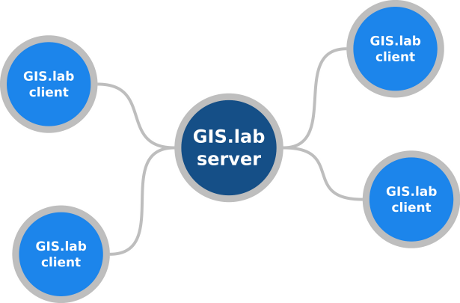
\includegraphics[keepaspectratio=true,height=0.6\textheight]{images/gislab-architecture.png}
	\end{center}
\end{frame}


\begin{frame}{Development}
	\textbf{Versions}
	\begin{itemize}
		\item currently preparing for 0.4 release
		\item general production release 0.5 in August 2014
	\end{itemize}

	\textbf{Authors}
	\begin{itemize}
		\item Marcel Dancák
		\item Ivan Minčík
	\end{itemize}

	\textbf{Sponsor}
	\begin{itemize}
		\item GISTA s.r.o.
	\end{itemize}
\end{frame}


\section{Installation}
\begin{frame}
	\begin{center}
		\LARGE\textbf{Installation}	
	\end{center}
\end{frame}


\begin{frame}{Requirements}
	\begin{itemize}
		\item server machines with Linux, Mac OX or Windows installed
		\item client machines with no OS \textbf{or} any OS installed
	\end{itemize}
\end{frame}


\begin{frame}{Installation in LAN - hard way}
	\textbf{Install dependencies}
	\begin{itemize}
		\item install VirtualBox, Vagrant, Git (optional)
	\end{itemize}

	\textbf{Install GIS.lab}
	\begin{itemize}
		\item \$ vagrant box add precise32-canonical http:// ...
		\item download installation ZIP \textbf{or} \$ git clone ...
		\item \$ vagrant up
	\end{itemize}
	\begin{flushleft}
		\textbf{\textcolor{Cyan}{25} minutes} \\
		\textbf{\textcolor{Cyan}{0} EUR} \\
	\end{flushleft}
\end{frame}


\begin{frame}{Installation in LAN - easy way - GIS.lab Unit}
	\begin{minipage}[\textheight]{\textwidth}
	\begin{columns}[T]
		\begin{column}{0.5\textwidth}
			\vspace{0.2\textheight}
			Plug-and-play
			\begin{flushleft}
				\textbf{\textcolor{Cyan}{5} minutes} \\
				\textbf{\textcolor{Cyan}{450} EUR} \\
			\end{flushleft}
		\end{column}
		\begin{column}{0.5\textwidth}
			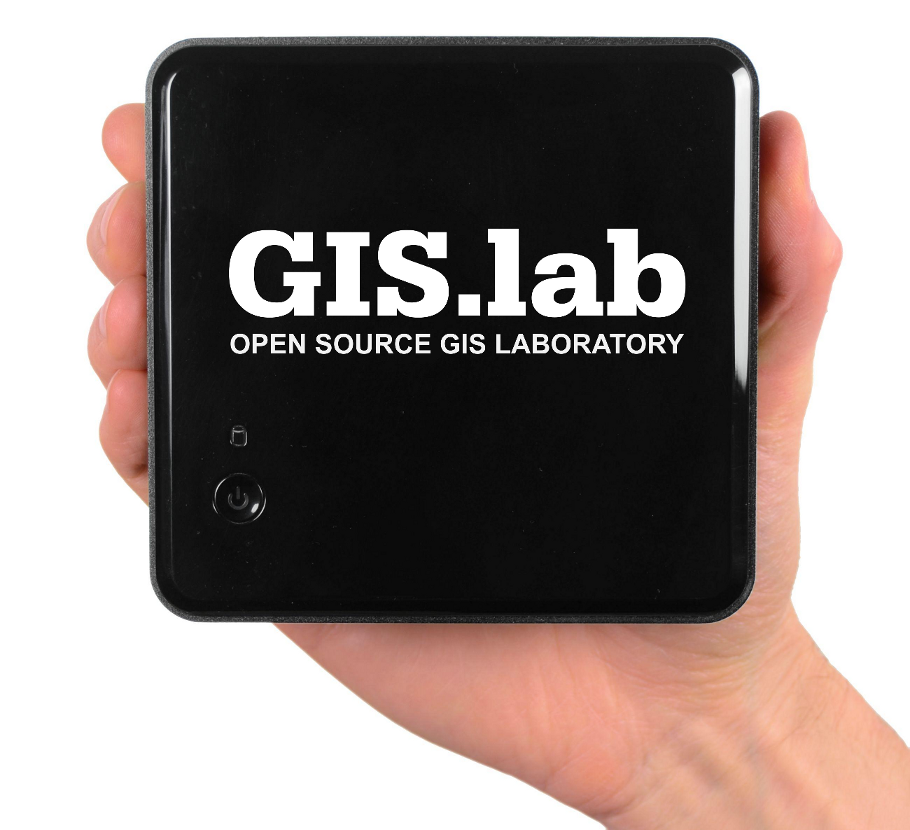
\includegraphics[keepaspectratio=true,width=\textwidth]{images/gislab-unit.png}
		\end{column}
	\end{columns}
	\end{minipage}
\end{frame}


\section{GIS.lab client}
\begin{frame}
	\begin{center}
		\LARGE\textbf{GIS.lab client}
	\end{center}
\end{frame}


\begin{frame}{Client modes}
	\textbf{Physical client}
	\begin{itemize}
		\item best performance
		\item original OS is temporary not available 
	\end{itemize}
	\begin{center}
		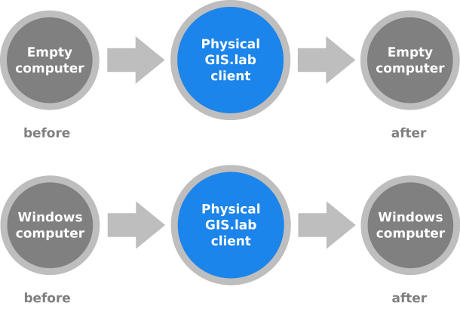
\includegraphics[keepaspectratio=true,height=0.6\textheight]{images/schema-physical-client.png}
	\end{center}
\end{frame}


\begin{frame}{Client modes}
	\textbf{Virtual client}
	\begin{itemize}
		\item lower performance
		\item original machine OS and GIS.lab client run side-by-side
	\end{itemize}
	\begin{center}
		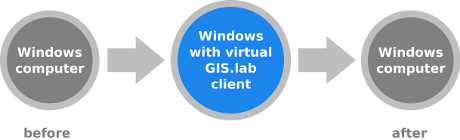
\includegraphics[keepaspectratio=true,height=0.4\textheight]{images/schema-virtual-client.png}
	\end{center}
\end{frame}


\begin{frame}{Client modes}
	\textbf{Other possibilities}
	\begin{itemize}
		\item third party LAN members (DHCP)
		\item Internet browsers (web.gis.lab)
	\end{itemize}
\end{frame}


\begin{frame}{Virtual client configuration}
	\begin{itemize}
		\item create new VirtualBox machine with no hard drive
		\item boot from network
	\end{itemize}
	\begin{center}
		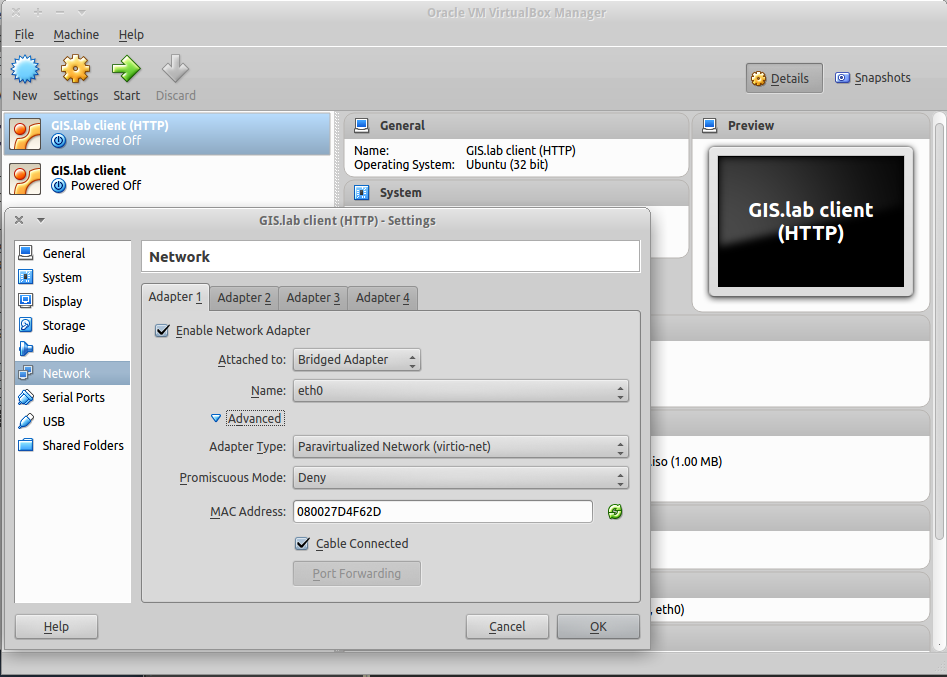
\includegraphics[keepaspectratio=true,height=0.6\textheight]{images/real-world-example/client-virtualbox-configuration.png}
	\end{center}
\end{frame}


\begin{frame}{Access policy by MAC}
	\textbf{config-user.cfg}
	\begin{itemize}
		\item GISLAB_UNKNOWN_MAC_POLICY=deny
		\item GISLAB_CLIENTS_ALLOWED=( 08:00:27:d4:f6:2d )
		\item \$ vagrant ssh -c "sudo gislab-allowmachines"
	\end{itemize}
	\begin{center}
		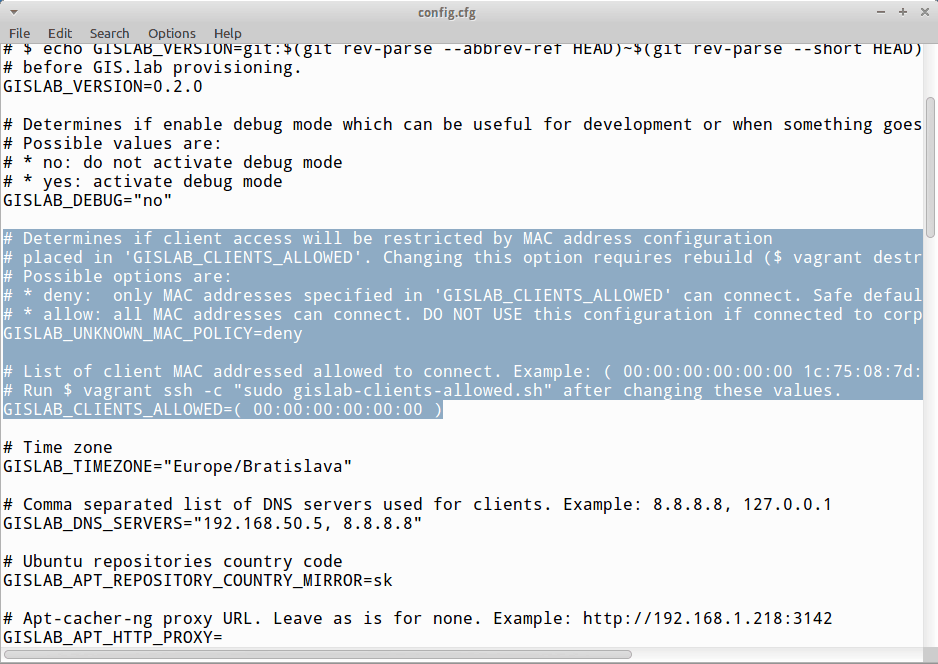
\includegraphics[keepaspectratio=true,height=0.5\textheight]{images/real-world-example/config-cfg.png}
	\end{center}
\end{frame}


\begin{frame}{Client login}
	\begin{center}
		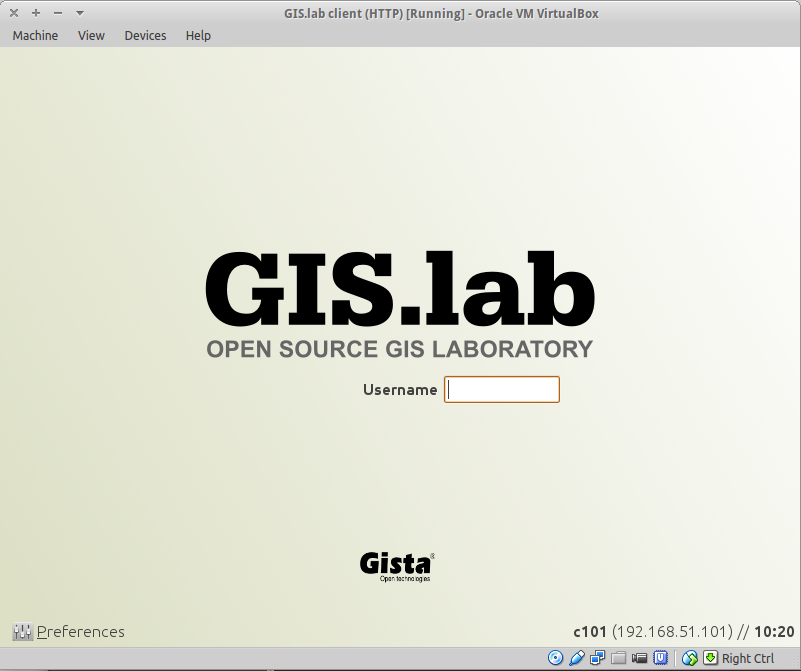
\includegraphics[keepaspectratio=true,height=0.7\textheight]{images/real-world-example/client-login.png}
	\end{center}
\end{frame}


\begin{frame}{Client desktop environment}
	\begin{center}
		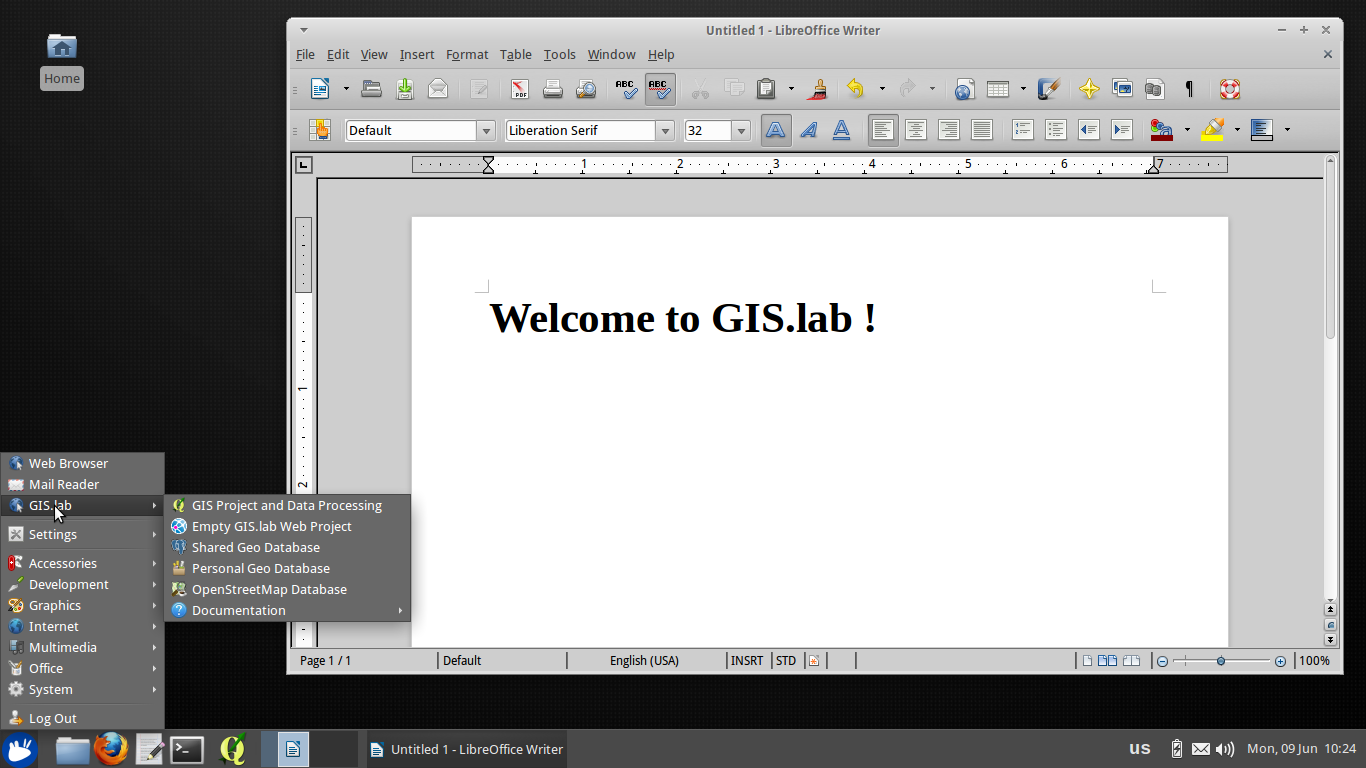
\includegraphics[keepaspectratio=true,height=0.7\textheight]{images/real-world-example/client-desktop-libreoffice.png}
	\end{center}
\end{frame}


\section{GIS project}
\begin{frame}
	\begin{center}
		\LARGE\textbf{Real world example}\normalsize

		\textbf{Urban planning map of city Banská Bystrica}
	\end{center}
\end{frame}


\begin{frame}{Spatial DB creation}
	\begin{itemize}
		\item create new SpatiaLite DB in SpatiaLite GUI
	\end{itemize}
	\begin{center}
		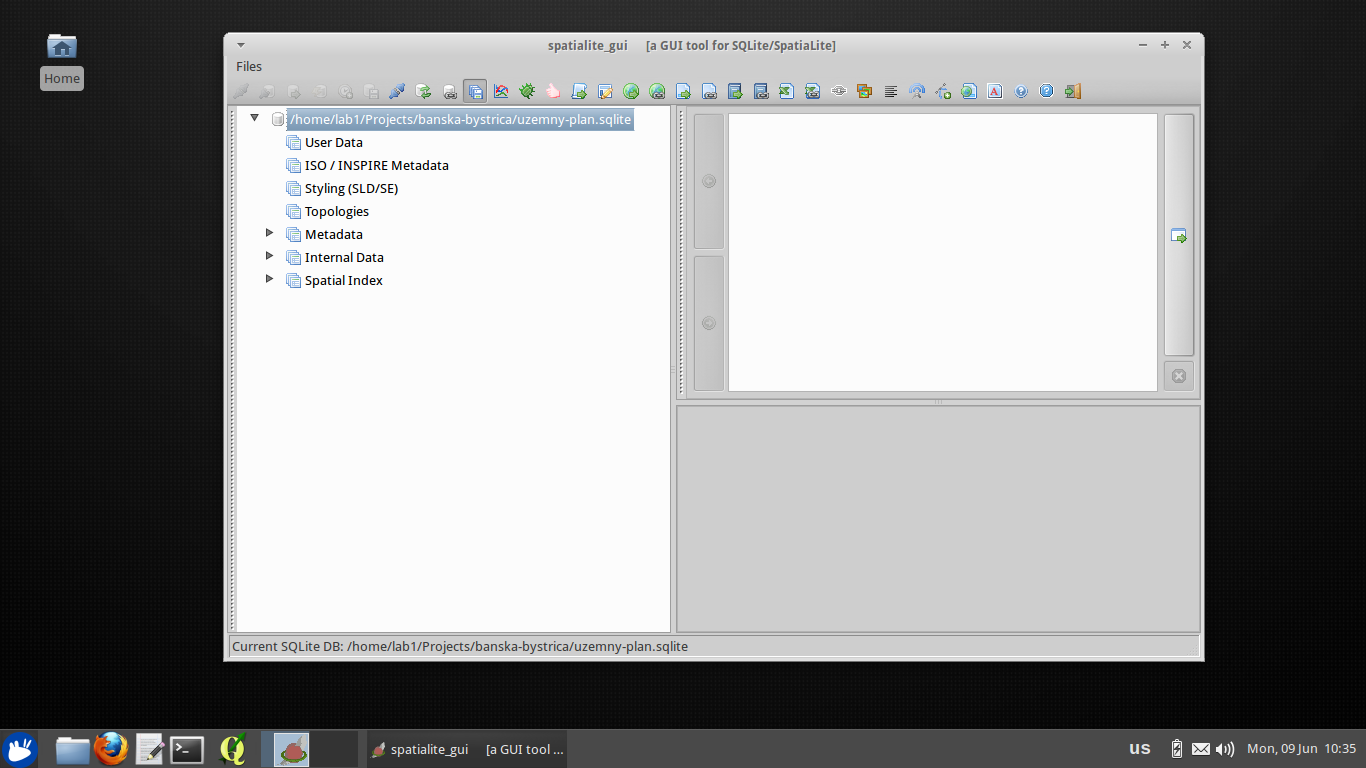
\includegraphics[keepaspectratio=true,height=0.7\textheight]{images/real-world-example/project-create-db.png}
	\end{center}
\end{frame}


\begin{frame}{Data import}
	\begin{itemize}
		\item inspect data in QGIS
		\item import layers to Spatialite DB using DB Manager plugin
	\end{itemize}
	\begin{center}
		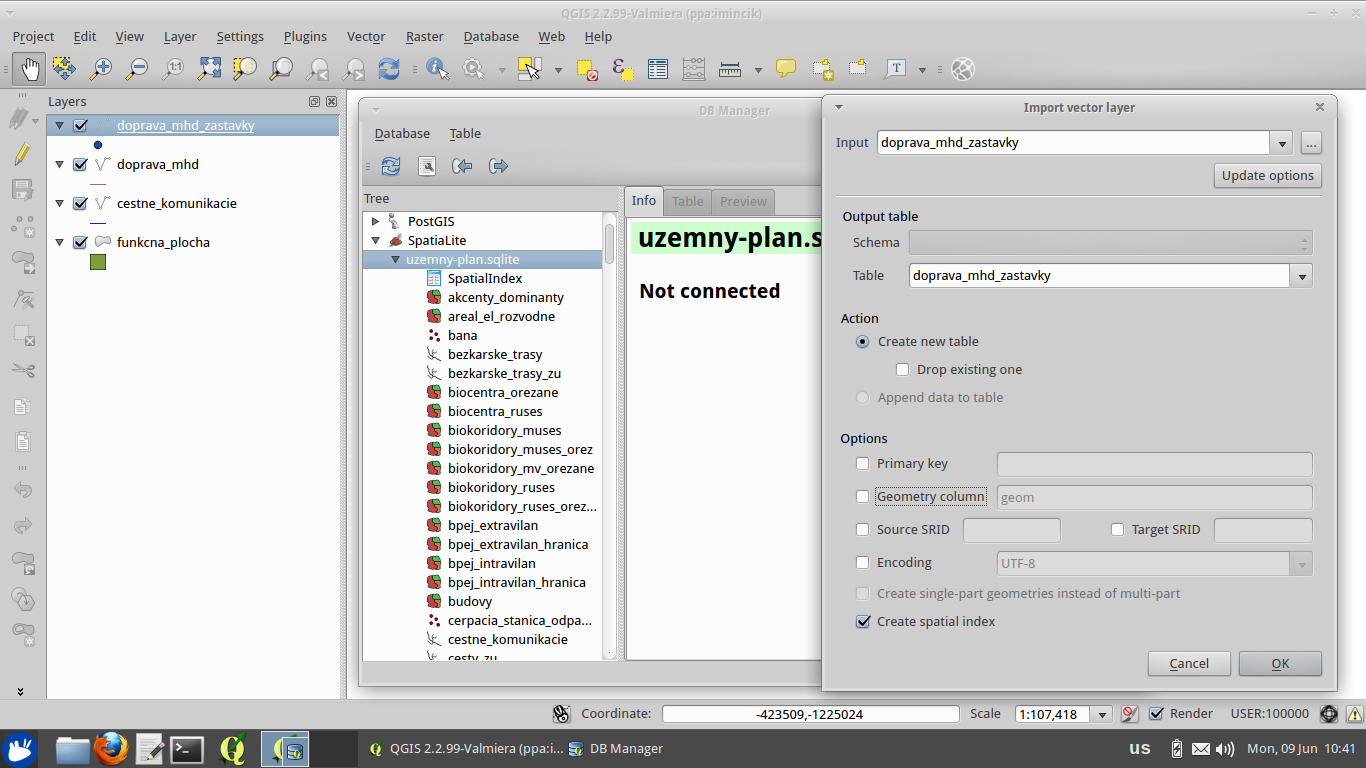
\includegraphics[keepaspectratio=true,height=0.6\textheight]{images/real-world-example/project-db-import-layers.png}
	\end{center}
\end{frame}


\begin{frame}{GIS project creation}
	\begin{itemize}
		\item load imported layers back from SpatiaLite DB to QGIS
	\end{itemize}
	\begin{center}
		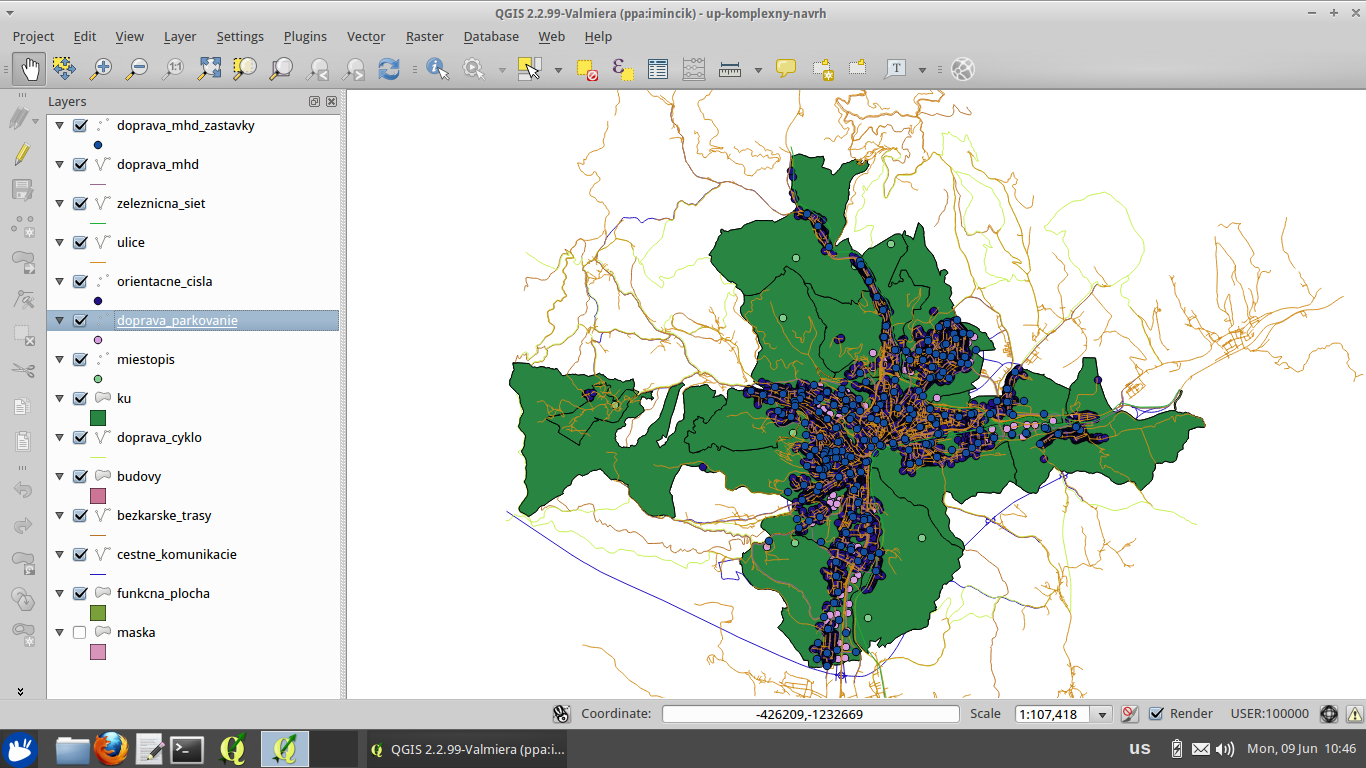
\includegraphics[keepaspectratio=true,height=0.6\textheight]{images/real-world-example/project-load-layers.png}
	\end{center}
\end{frame}


\begin{frame}{TOC structure}
	\begin{itemize}
		\item create layer groups
		\item rename layers and move to corresponding groups
	\end{itemize}
	\begin{center}
		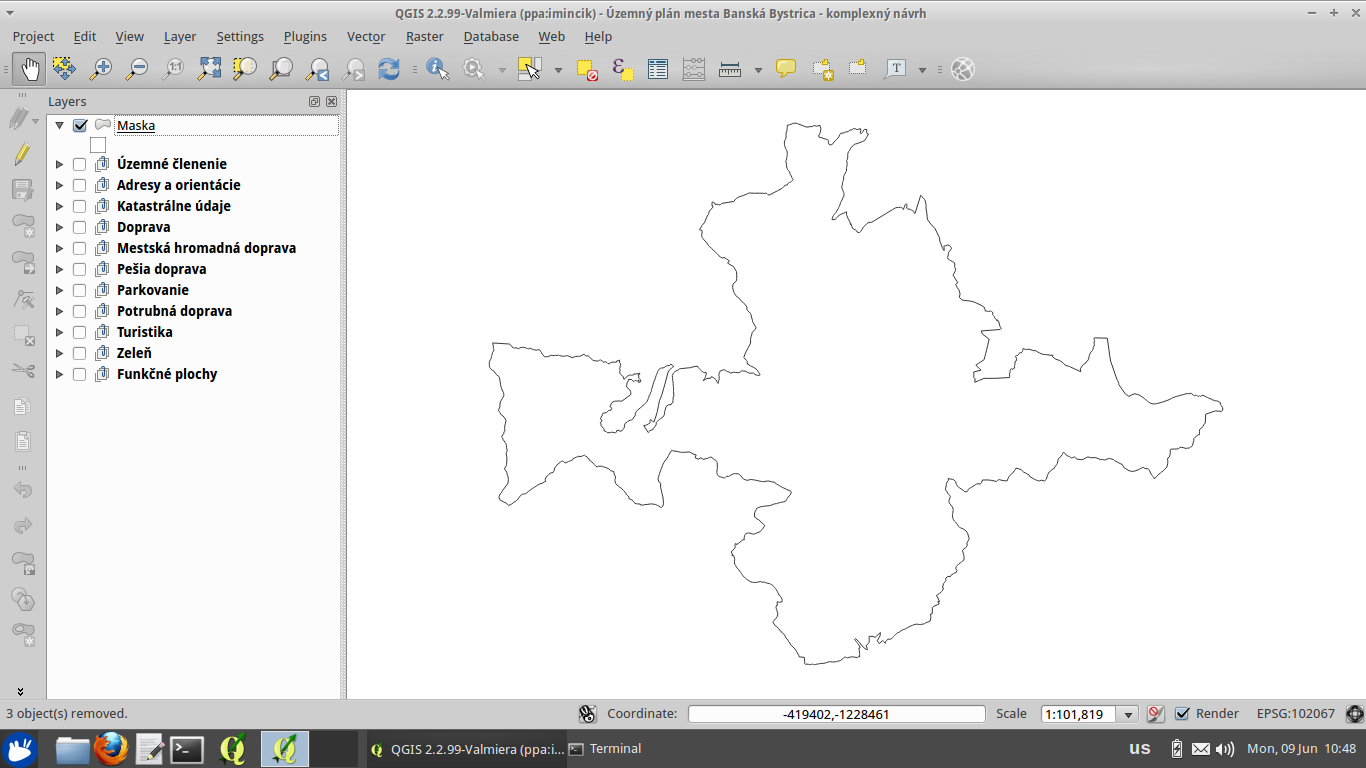
\includegraphics[keepaspectratio=true,height=0.6\textheight]{images/real-world-example/project-create-layer-groups.png}
	\end{center}
\end{frame}


\begin{frame}{Layers styling}
	\begin{itemize}
		\item assign styles and map symbols to each layer
		\item categorize layer by attribute values
	\end{itemize}
	\begin{center}
		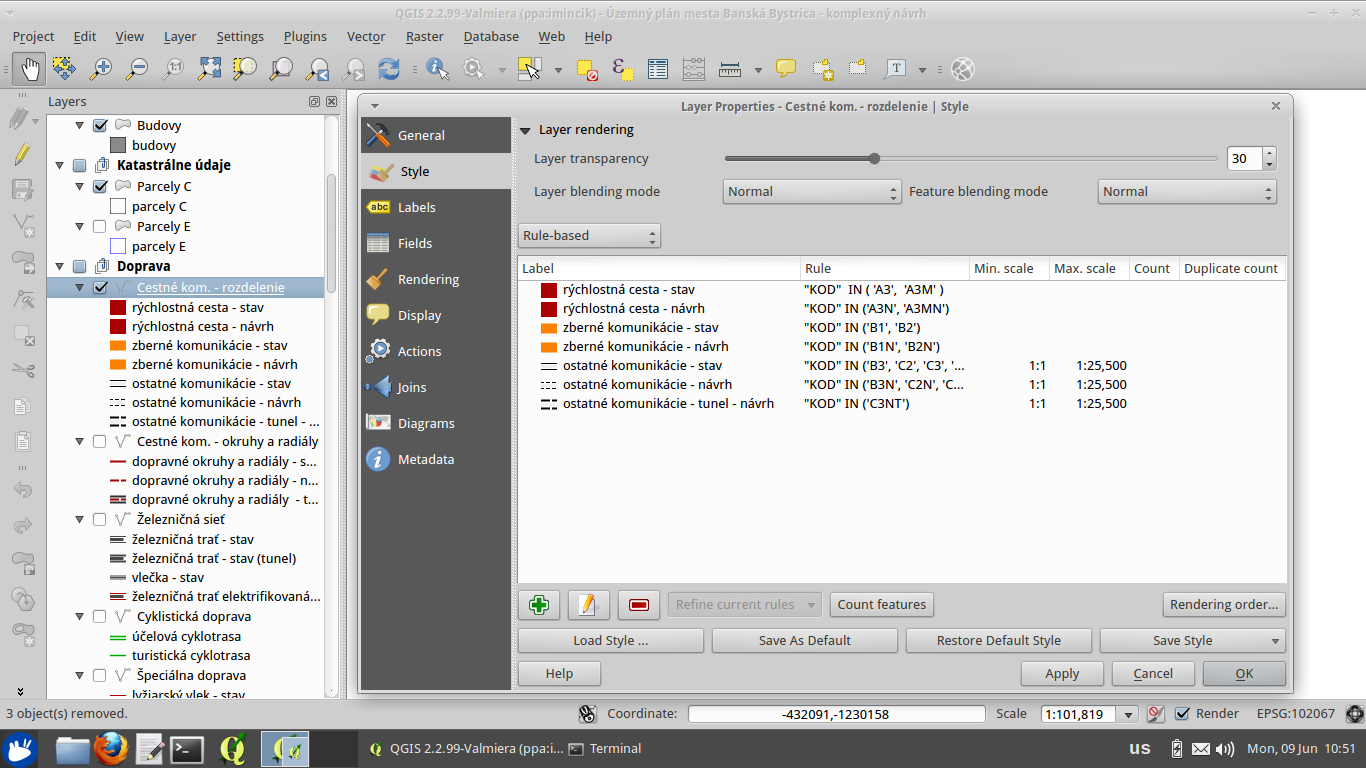
\includegraphics[keepaspectratio=true,height=0.6\textheight]{images/real-world-example/project-layer-style.png}
	\end{center}
\end{frame}


\begin{frame}{Layers styling}
	\begin{center}
		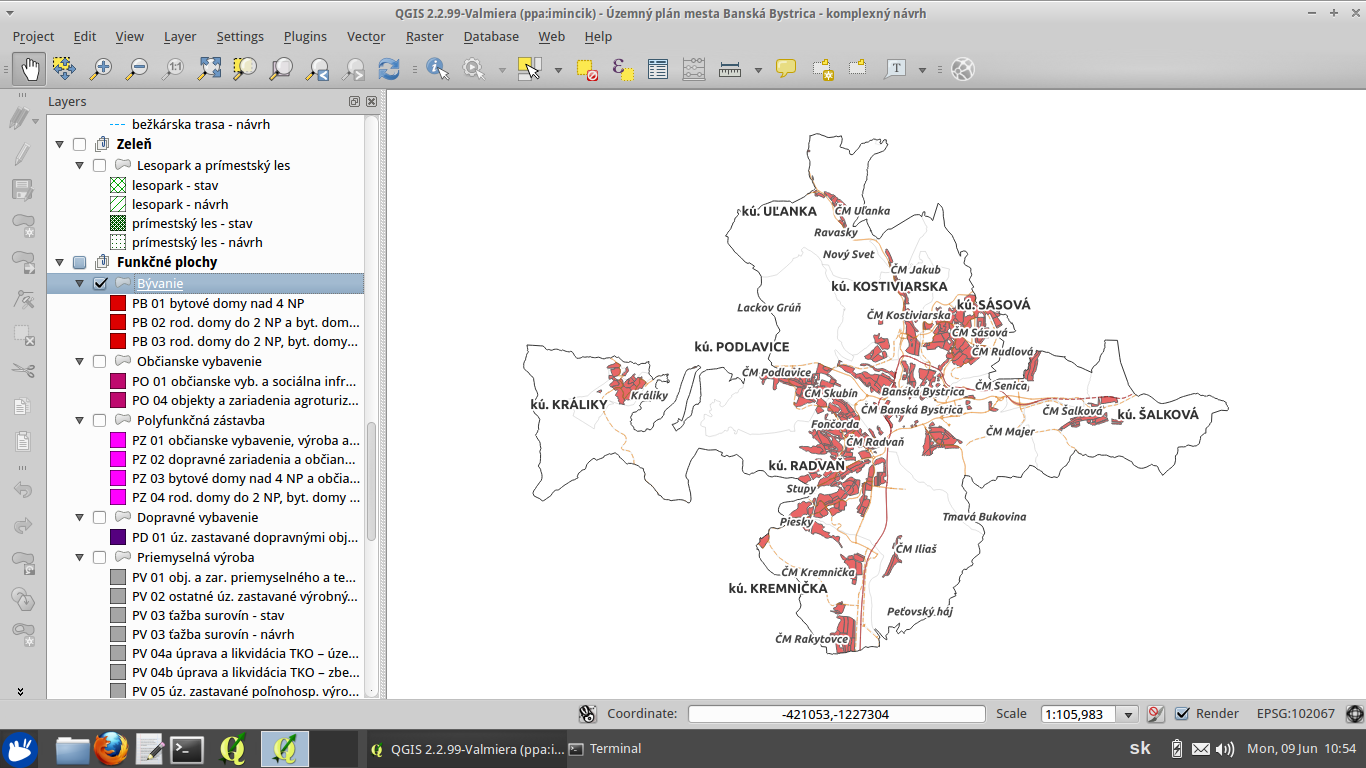
\includegraphics[keepaspectratio=true,height=0.6\textheight]{images/real-world-example/project-layer-style-ready.png}
	\end{center}
\end{frame}


\begin{frame}{Attributes}
	\begin{itemize}
		\item assign human names to attribute fields
		\item create attribute form
	\end{itemize}
	\begin{center}
		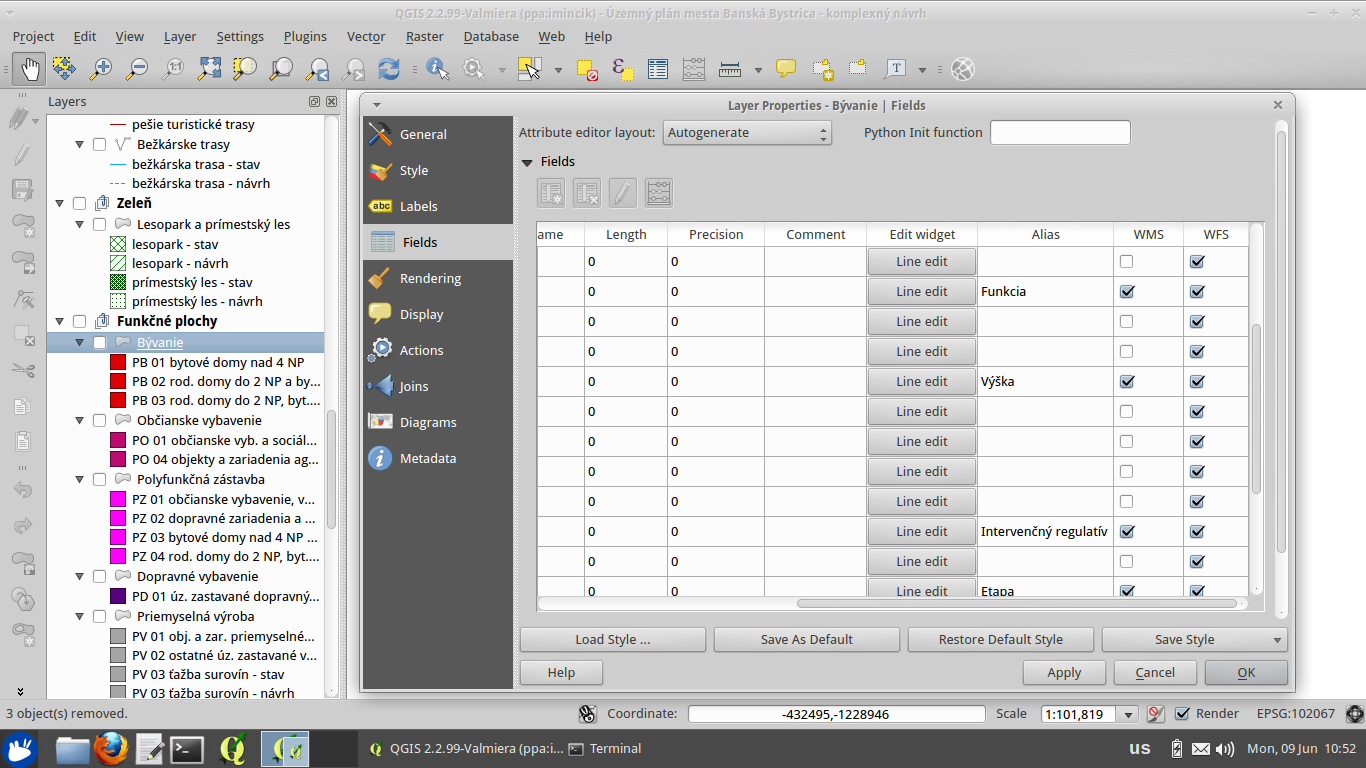
\includegraphics[keepaspectratio=true,height=0.6\textheight]{images/real-world-example/project-layer-attributes.png}
	\end{center}
\end{frame}


\begin{frame}{Feature information}
	\begin{itemize}
		\item configure layers with activated feature info
	\end{itemize}
	\begin{center}
		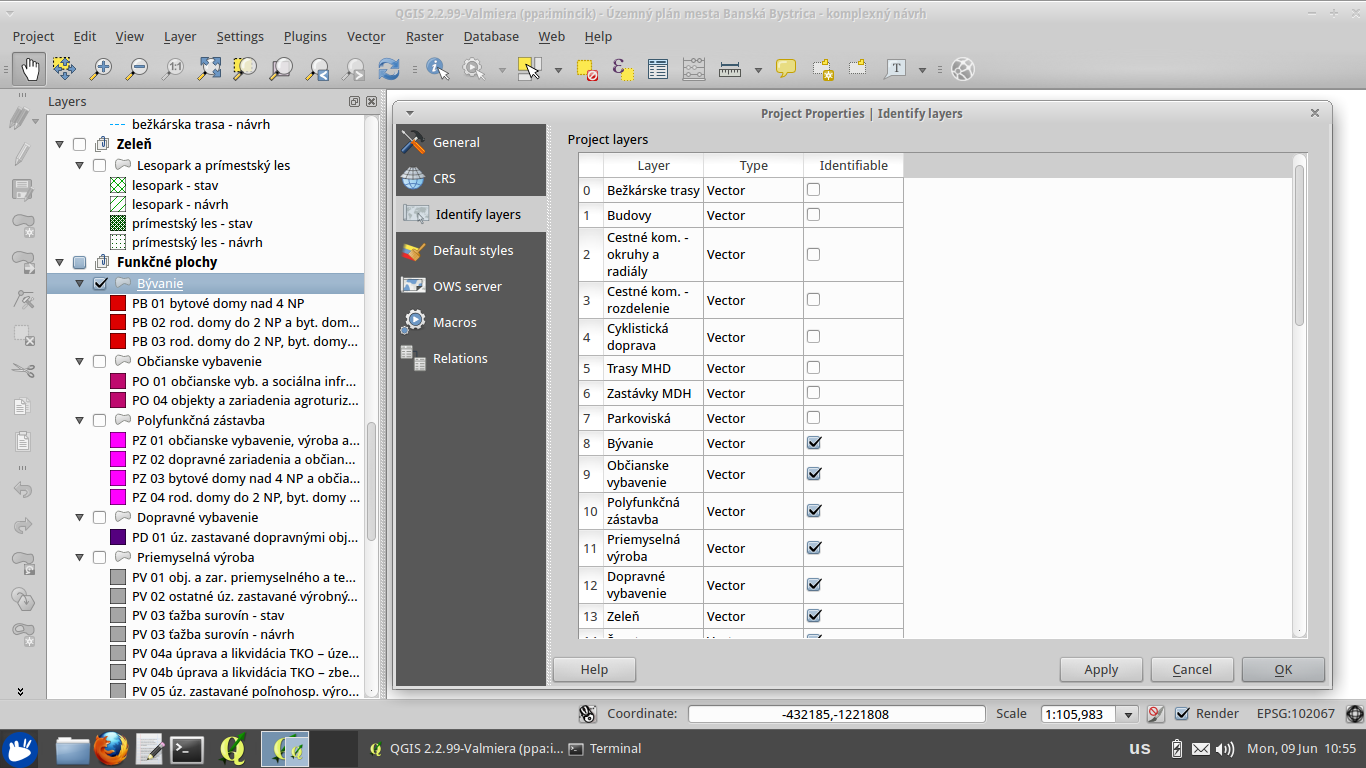
\includegraphics[keepaspectratio=true,height=0.6\textheight]{images/real-world-example/project-feature-info.png}
	\end{center}
\end{frame}


\begin{frame}{Project properties}
	\begin{itemize}
		\item assign project title, abstract, author name and email
	\end{itemize}
	\begin{center}
		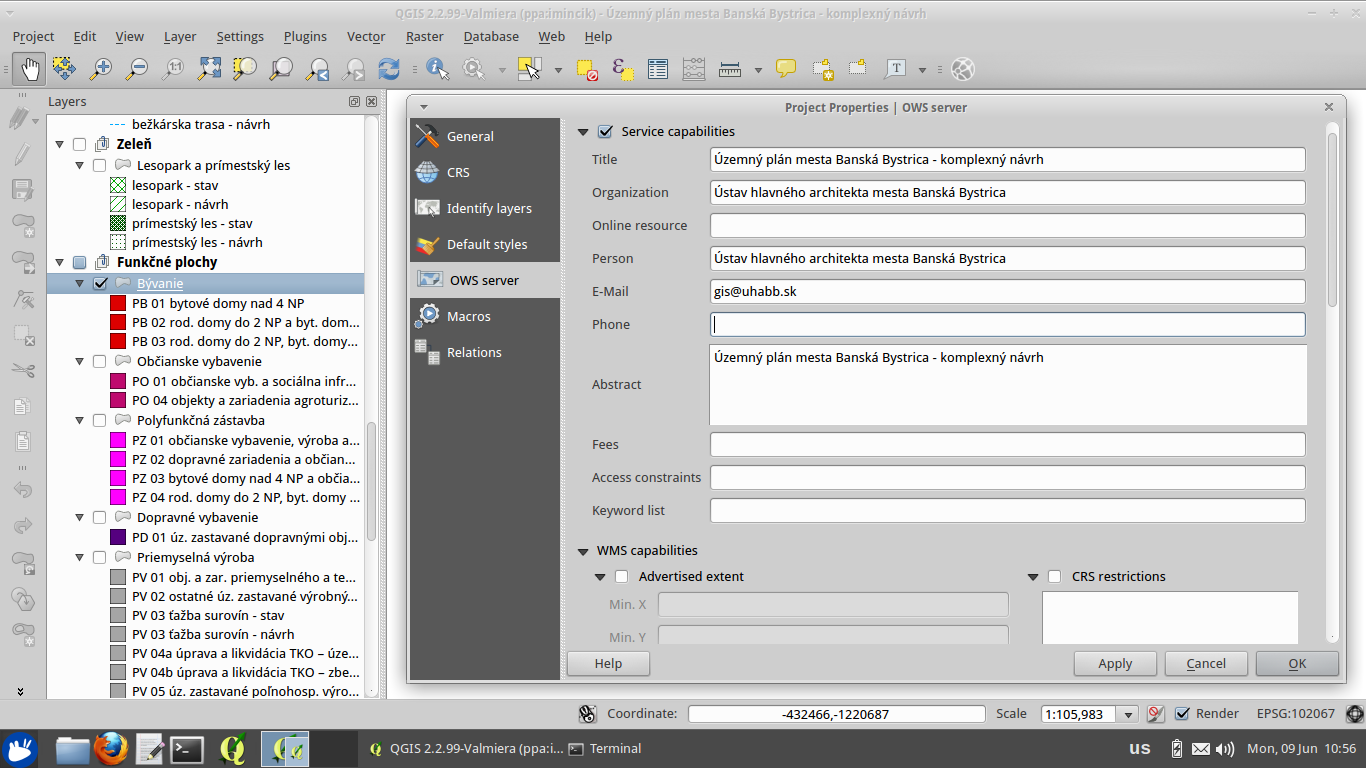
\includegraphics[keepaspectratio=true,height=0.6\textheight]{images/real-world-example/project-properties.png}
	\end{center}
\end{frame}


\begin{frame}{Project publishing}
	\begin{itemize}
		\item save project
		\item move project to Share/\$USER directory
	\end{itemize}
	\begin{center}
		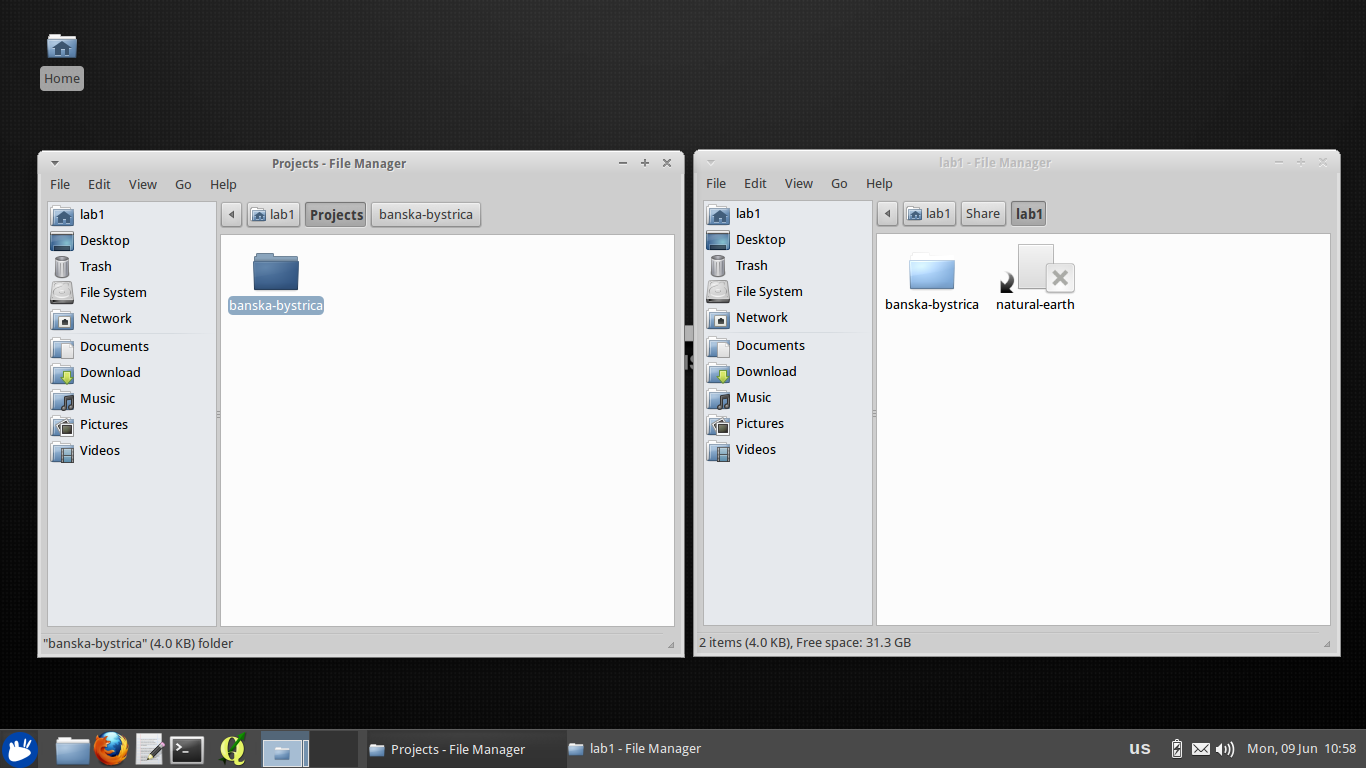
\includegraphics[keepaspectratio=true,height=0.6\textheight]{images/real-world-example/project-share-directory.png}
	\end{center}
\end{frame}


\begin{frame}{Project publishing}
	\begin{itemize}
		\item publish project in GIS.lab Web
	\end{itemize}
	\begin{center}
		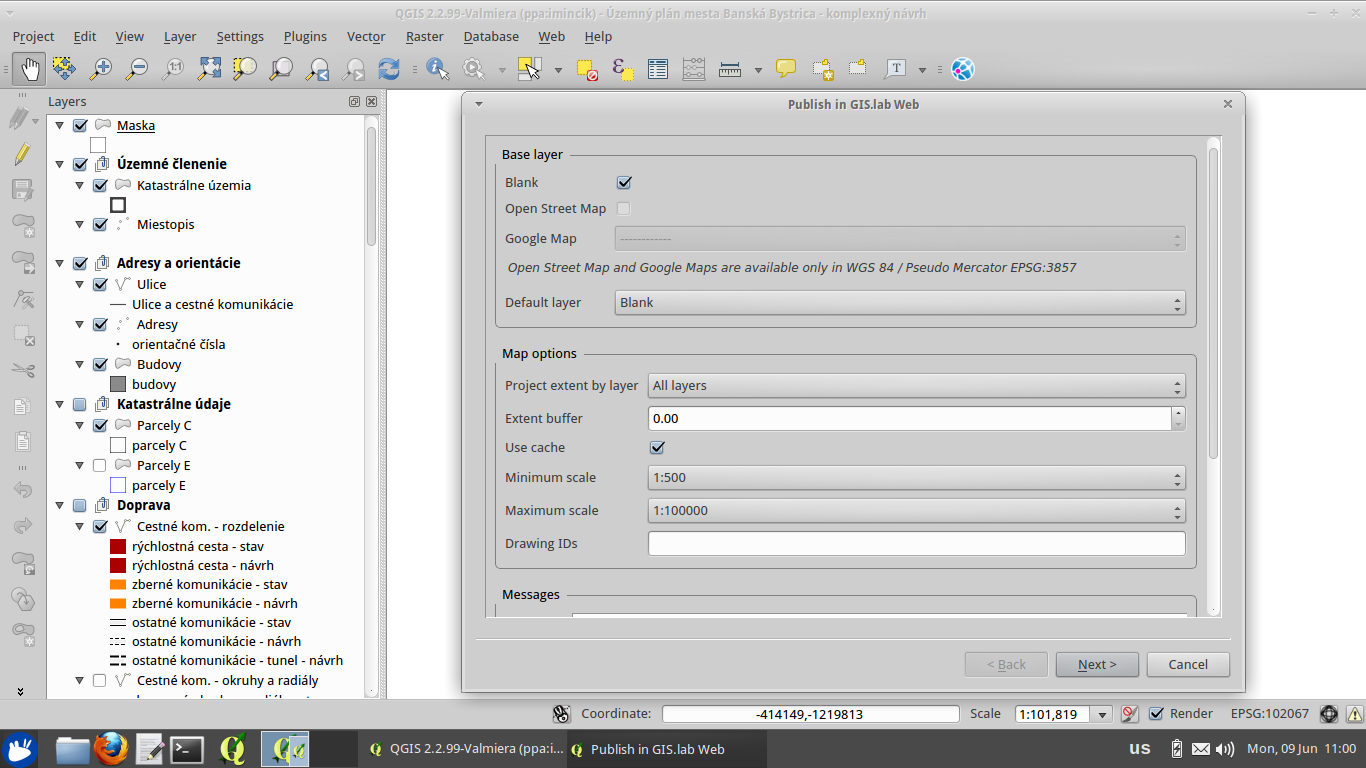
\includegraphics[keepaspectratio=true,height=0.6\textheight]{images/real-world-example/project-publish.png}
	\end{center}
\end{frame}


\section{GIS.lab Web}
\begin{frame}
	\begin{center}
		\LARGE\textbf{GIS.lab Web}
	\end{center}
\end{frame}


\begin{frame}{GIS.lab Web}
	\textbf{http://web.gis.lab/?PROJECT=path-to-project}
	\begin{center}
		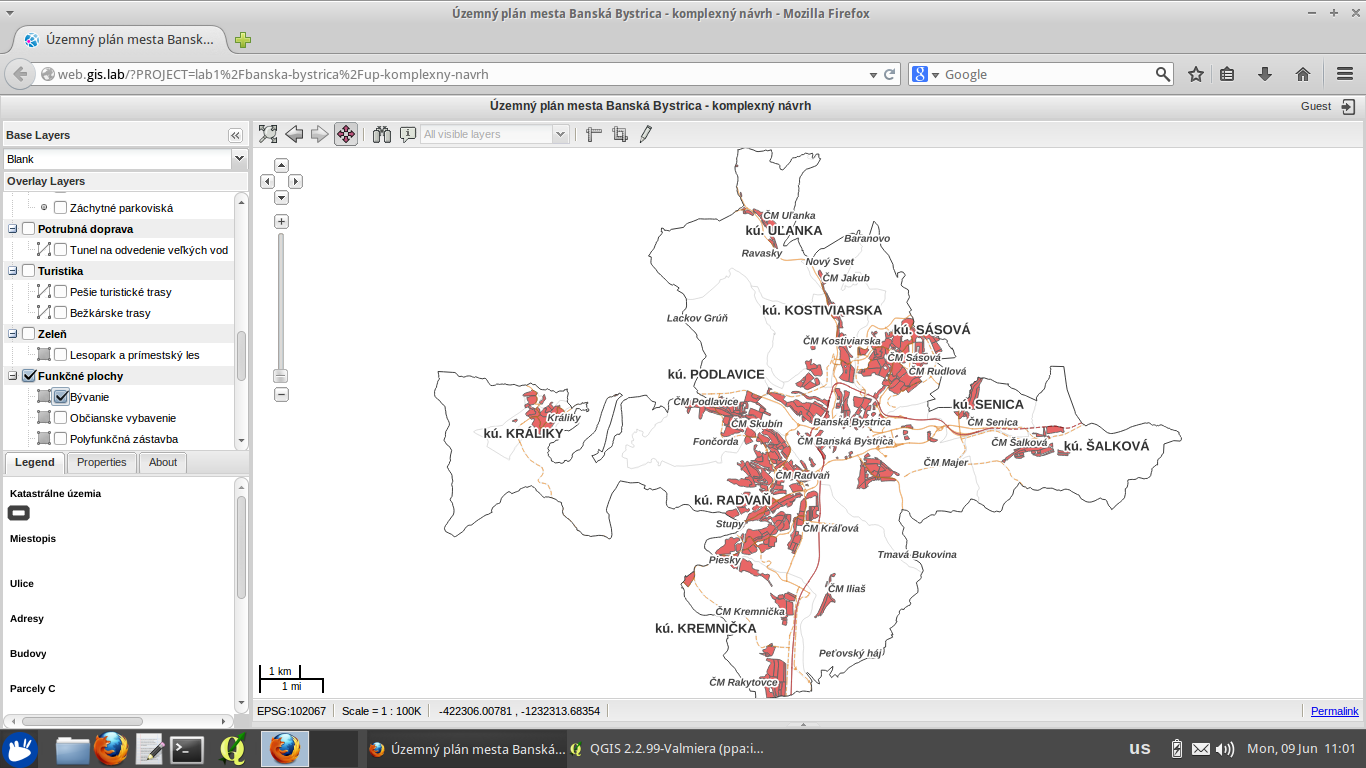
\includegraphics[keepaspectratio=true,height=0.7\textheight]{images/real-world-example/project-gislab-web.png}
	\end{center}
\end{frame}


\begin{frame}{GIS.lab Web}
	\begin{itemize}[<+->]
		\item base layers (WMS, OSM, Google), overlay layers from QGIS project
		\item measure lines and polygons
		\item feature information and advanced search
		\item drawing new POINTS, LINES, POLYGONS with attributes
		\item drawing patches to overlay layer's features
		\item print output creation
		\item permalink
		\item intelligent automatic caching
	\end{itemize}
\end{frame}


\begin{frame}{GIS.lab Web search}
	\begin{center}
		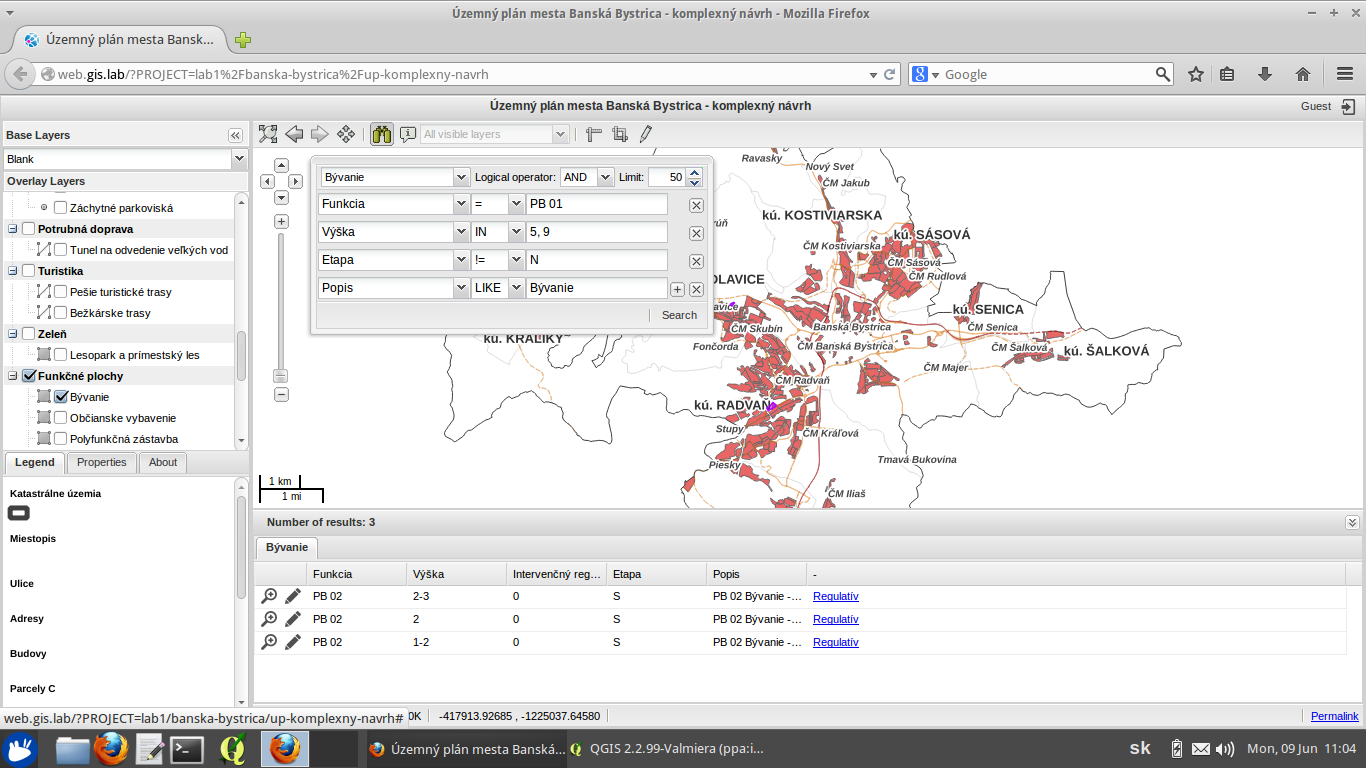
\includegraphics[keepaspectratio=true,height=0.7\textheight]{images/real-world-example/project-gislab-web-search.png}
	\end{center}
\end{frame}


\begin{frame}{GIS.lab Web drawing}
	\begin{center}
		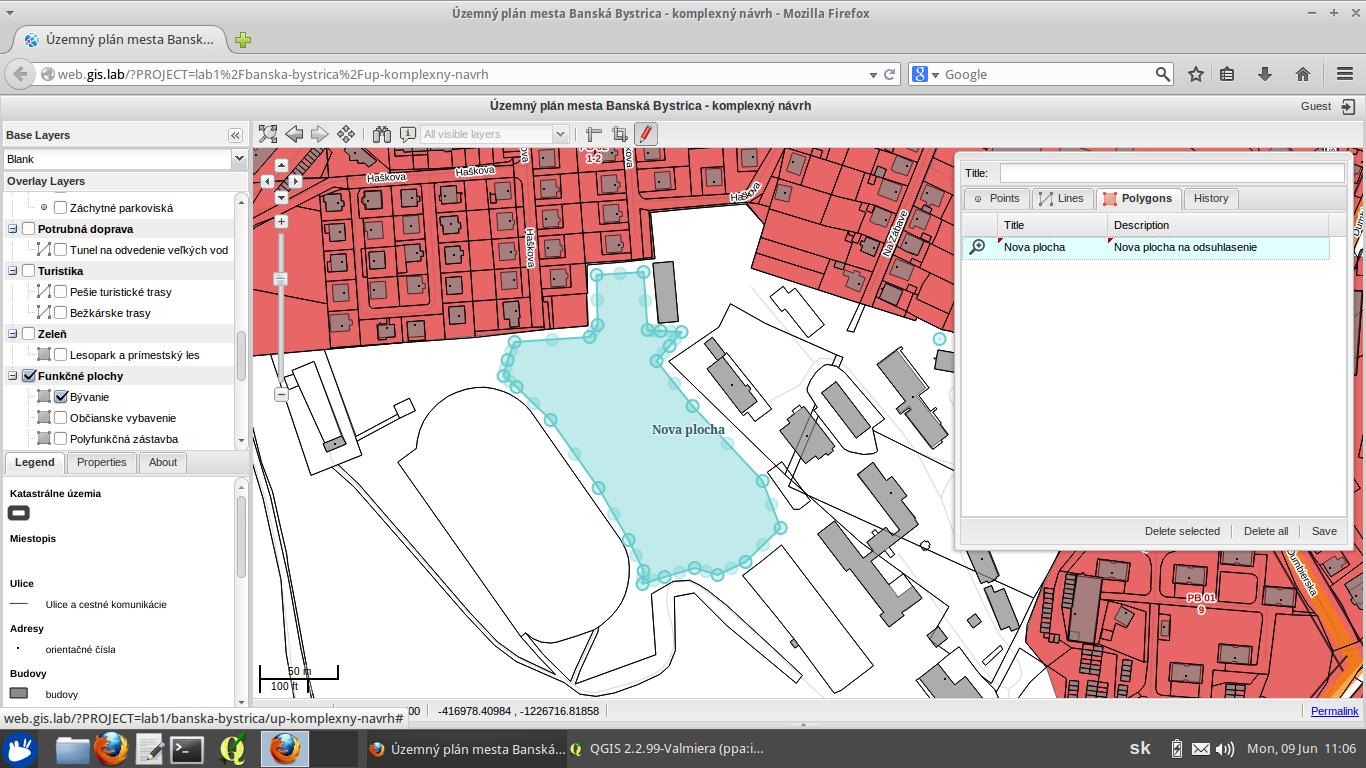
\includegraphics[keepaspectratio=true,height=0.7\textheight]{images/real-world-example/project-gislab-web-drawing.png}
	\end{center}
\end{frame}


\section{Amazon AWS}
\begin{frame}
	\begin{center}
		\LARGE\textbf{Amazon AWS provider}
	\end{center}
\end{frame}


\begin{frame}{Installation in Amazon AWS}
	\textbf{Install dependencies}
	\begin{itemize}
		\item \$ vagrant plugin install vagrant-aws
	\end{itemize}

	\textbf{config-user.cfg}
	\begin{itemize}
		\item configure Amazon credentials, placement and security zone
	\end{itemize}

	\textbf{Install GIS.lab server}
	\begin{itemize}
		\item \$ vagrant up --provider=aws
	\end{itemize}
	
	\begin{flushleft}
		\textbf{\textcolor{Cyan}{5} minutes} \\
		\textbf{\textcolor{Cyan}{200} EUR / month} \\
	\end{flushleft}
\end{frame}


\begin{frame}{GIS.lab Web in Amazon AWS}
	\begin{itemize}
		\item copy project files on AWS server
	\end{itemize}
	\begin{center}
		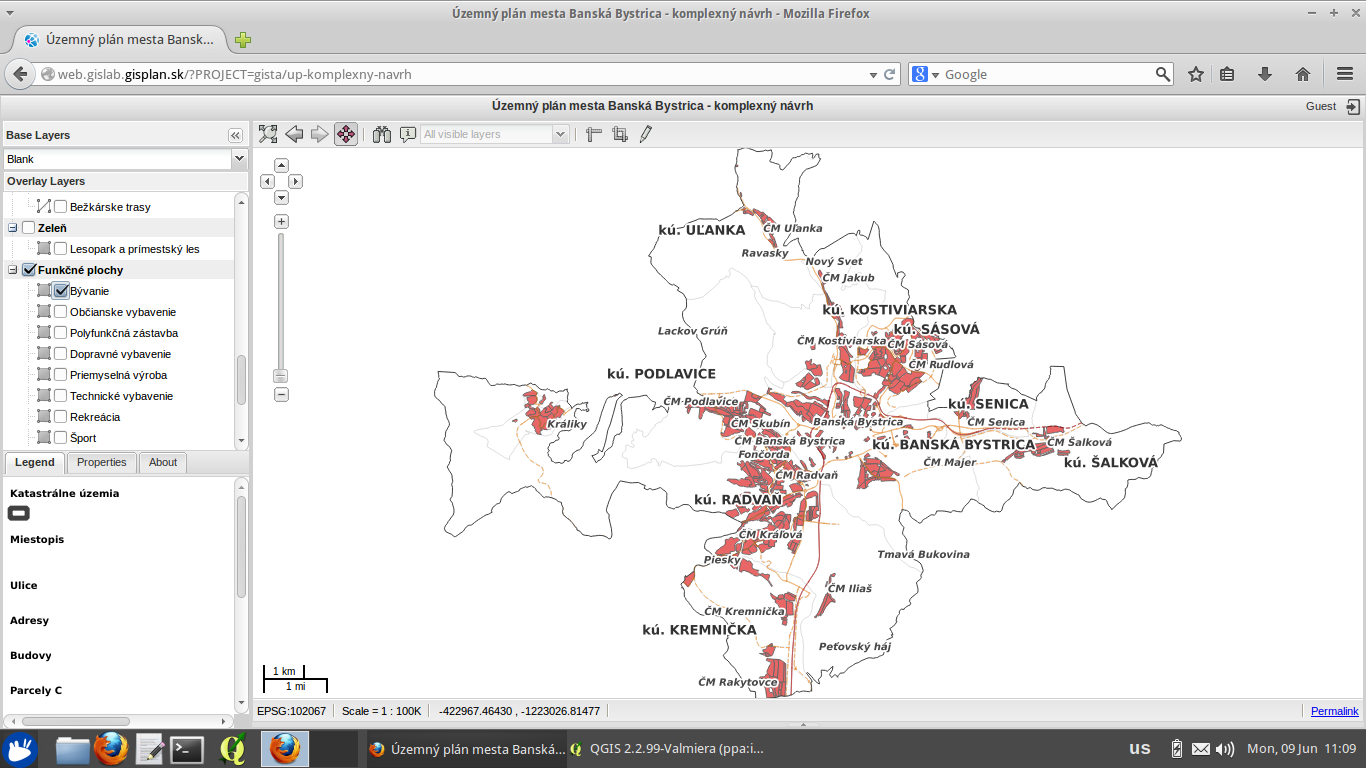
\includegraphics[keepaspectratio=true,height=0.7\textheight]{images/real-world-example/project-gislab-web-amazon-aws.png}
	\end{center}
\end{frame}


\section{Future plans}
\begin{frame}
	\begin{center}
		\LARGE\textbf{Future plans}
	\end{center}
\end{frame}


\begin{frame}{Future plans}
	\begin{itemize}
		\item web management interface
		\item multiple templates for GIS.lab Web
		\item GIS.lab Web interface for mobile devices
		\item GIS.lab Workstation
		\item Docker
		\item load balanced cluster
		\item decentralized GIS.lab network
		\item test suite - GIS software stack, GIS.lab services and features
	\end{itemize}
\end{frame}


\section{Final notes}
\begin{frame}
	\begin{center}
		\LARGE\textbf{Final notes}
	\end{center}
\end{frame}


\begin{frame}{Where to use GIS.lab ?}
	\begin{itemize}
		\item virtual desktop infrastructure for LAN
		\item public map service in cloud
		\item crowd mapping
		\item development and testing environment
		\item education and Open Source GIS software advocacy
		\item rapid deployment of crisis management command center with spatial support
	\end{itemize}
\end{frame}


\begin{frame}{Final notes}
	We are looking forward to welcome new users, testers and developers.
	
	\bigskip
	http://imincik.github.io/gis-lab
	
	\bigskip
	Thanks for attention.
	
	Ivan Minčík, ivan.mincik@gmail.com

	\bigskip 
	\LARGE\textbf{Questions ?}
\end{frame}


% document END
\end{document}